\documentclass[../../main.tex]{subfiles}
% \documentclass[a4paper,10pt]{ltjsarticle}
\begin{document}
\rhead{京都大学後期$1993$年$2$番}
\setcounter{equation}{0}
\begin{oframed}
  \subfile{problem}
\end{oframed}
\setlength{\columnseprule}{0.4pt}
\begin{multicols}{2}
  {\bf [解答]}
  $f(x)=x^3-3ax$の一階微分は
  \begin{align}
    f'(x)=3(x^2-a)
  \end{align}
  だから，$a\le 0$の時$f'(x)\ge 0$となり$f(x)$は単調増加である．
  よってこの時$f(x)=t$は一つしか解を持たず，題意の条件を満たさない．

  そこで以下
  \begin{align}
    a > 0
  \end{align}
  として考える．
  $f(x)$の増減表は\cref{1993-2:table:1}となる．

  \begin{table}[H]
    \centering
    \caption{$f(x)$の増減表}
    \label{1993-2:table:1}
    \begin{tabular}{|c||c|c|c|c|c|}
      \hline
      $x$  & $\cdots$   & $-\sqrt{a}$  & $\cdots$   & $\sqrt{a}$    & $\cdots$   \\
      \hline
      $f'$ & $+$        & $0$          & $-$        & $0$           & $+$        \\
      \hline
      $f$  & $\nearrow$ & $2a\sqrt{a}$ & $\searrow$ & $-2a\sqrt{a}$ & $\nearrow$ \\
      \hline
    \end{tabular}
  \end{table}

  従って，$y=f(x)$のグラフは\cref{1993-2:fig:1}のようになる．
  \begin{figure}[H]
    \centering
    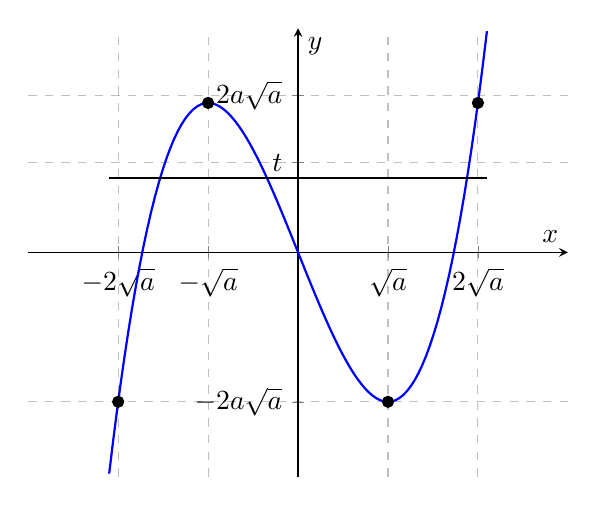
\begin{tikzpicture}
      \begin{axis}[
          axis lines=middle,
          xlabel=$x$,
          ylabel=$y$,
          xmin=-3, xmax=3,
          ymin=-3, ymax=3,
          xtick={-2,-1,0,1,2},
          ytick={-2,1.2,2.1},
          xticklabels={$-2\sqrt{a}$, $-\sqrt{a}$, $0$, $\sqrt{a}$, $2\sqrt{a}$},
          yticklabels={$-2a\sqrt{a}$,$t$, $2a\sqrt{a}$},
          grid=both, % グリッド線を表示
          grid style={dashed, gray!50}, % グリッド線のスタイル
          clip = false,
          %xlabel style={at={(axis description cs:1,0)},anchor=north west},
          %ylabel style={at={(axis description cs:0,1)},anchor=south east}
        ]

        % a=1のときの関数 y = x^3 - 3x をプロット
        \addplot[domain=-2.1:2.1, samples=100, blue, thick]{x^3 - 3*x};
        \addplot[domain=-2.1:2.1, samples=100, black, thick]{1};
        \addplot[only marks,mark=*] coordinates {(1, -2)};
        \addplot[only marks,mark=*] coordinates {(-1, 2)};
        \addplot[only marks,mark=*] coordinates {(2, 2)};
        \addplot[only marks,mark=*] coordinates {(-2, -2)};
      \end{axis}
    \end{tikzpicture}
    \caption{$y=f(x)$の概形}
    \label{1993-2:fig:1}
  \end{figure}

  $f(x)=t$ の解が $y=f(x)$ と $y=t$ の交点の $x$ 座標に対応していることから
  $f(x)=t$が三つの解を持つ条件は
  \begin{align}
    a>0 \land -2a\sqrt{a} < t < 2a\sqrt{a}
  \end{align}
  である．$\cdots$(答)

  \vspace{10pt}

  \paragraph{(2)}
  (1)の考察から，$a \le 0$の時，$f(x)$は単調増加であるから，
  $g(x) = f(f(x))$も単調増加となり，$g(x)=0$が9つの異なる実数解を持つことはない．
  従って
  \begin{align}
    a > 0
  \end{align}
  が必要．以下この条件で考える．

  $X=f(x)$とおくと，$g(x)=0$はすなわち$f(X)=0$であるから，
  $y=f(X)$のグラフを考えると，(1)と同様に\cref{1993-2:fig:2}のようになる．

  \begin{figure}[H]
    \centering
    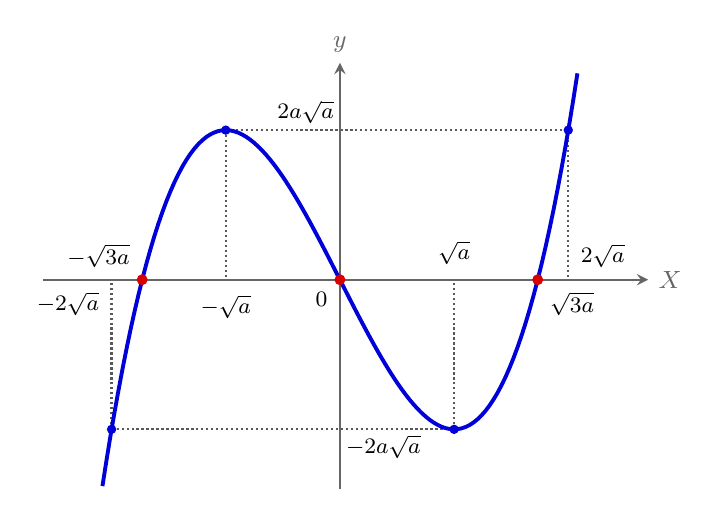
\begin{tikzpicture}[x=1.45cm, y=0.95cm, >=stealth,
      every node/.style={font=\small}]
      % a=1 として y = X^3 - 3X を描く（目盛りは一般の a で表記）．
      \pgfmathsetmacro{\rt}{sqrt(3)}
      \coordinate (Pmax) at (-1, 2);
      \coordinate (Pmin) at (1, -2);
      \coordinate (Lend) at (-2, -2);
      \coordinate (Rend) at (2, 2);
      % 補助線（極値・端点から座標軸へ）
      \draw[densely dotted, thick, gray!70!black] (Pmax) -- (-1, 0);
      \draw[densely dotted, thick, gray!70!black] (Pmin) -- (1, 0);
      \draw[densely dotted, thick, gray!70!black] (Lend) -- (-2, 0);
      \draw[densely dotted, thick, gray!70!black] (Rend) -- (2, 0);
      \draw[densely dotted, thick, gray!70!black] (Pmax) -- (Rend);
      \draw[densely dotted, thick, gray!70!black] (Lend) -- (Pmin);
      % 座標軸
      \draw[->, thick, gray!80!black] (-2.6, 0) -- (2.7, 0) node[right] {$X$};
      \draw[->, thick, gray!80!black] (0, -2.8) -- (0, 2.9) node[above] {$y$};
      % y = f(X)
      \draw[line width=1.4pt, blue!85!black, domain=-2.08:2.08, samples=120]
      plot (\x, {\x*\x*\x - 3*\x});
      % 目盛り（隣接するものは軸の上下に振り分ける）
      \node[below left=1pt, font=\footnotesize] at (-2, 0) {$-2\sqrt{a}$};
      \node[above left=1pt, font=\footnotesize] at (-\rt, 0) {$-\sqrt{3a}$};
      \node[below=2pt, font=\footnotesize] at (-1, 0) {$-\sqrt{a}$};
      \node[below left=1pt, font=\footnotesize] at (0, 0) {$0$};
      \node[above=2pt, font=\footnotesize] at (1, 0) {$\sqrt{a}$};
      \node[below right=1pt, font=\footnotesize] at (\rt, 0) {$\sqrt{3a}$};
      \node[above right=1pt, font=\footnotesize] at (2, 0) {$2\sqrt{a}$};
      \node[above left=1pt, fill=white, inner sep=1pt, font=\footnotesize] at (0, 2) {$2a\sqrt{a}$};
      \node[below right=1pt, fill=white, inner sep=1pt, font=\footnotesize] at (0, -2) {$-2a\sqrt{a}$};
      % 極値・端点
      \foreach \p in {Pmax, Pmin, Lend, Rend} {
        \node[circle, fill=blue!85!black, inner sep=1.2pt] at (\p) {};
      }
      % f(X) = 0 の解
      \foreach \x in {-\rt, 0, \rt} {
        \node[circle, fill=red!85!black, inner sep=1.4pt] at (\x, 0) {};
      }
    \end{tikzpicture}
    \caption{$y=f(X)$の概形}
    \label{1993-2:fig:2}
  \end{figure}

  $f(x)$ は3次関数であるから$f(x)=t$ をみたす $x$ は高々3つしかないこととグラフの概形から，
  $f(X)=0$の3つの解
  \begin{align}
    X = 0, \pm \sqrt{3a}
  \end{align}
  にそれぞれ3つずつの $x$ が対応している時のみ, $f(f(x))=0$ は9つの異なる実数解を持つ.
  (1)の結果から，求める条件は$a>0$の元で
  \begin{align}
    -2a\sqrt{a} < -\sqrt{3a}, \sqrt{3a} < 2a\sqrt{a}
    \quad \therefore
    a > \dfrac{\sqrt{3}}{2}
  \end{align}
  である．これは$a>0$を満たしているから，求める条件は
  \begin{align}
    a > \dfrac{\sqrt{3}}{2}
  \end{align}
  である．$\cdots$(答)

  \vspace{10pt}

  {\bf [解説]}

  \newpage
\end{multicols}
\end{document}
